\documentclass[tikz,border=12pt]{standalone}
\usepackage[T1]{fontenc}
\usepackage{lmodern}
\usetikzlibrary{positioning,arrows.meta,shapes.geometric,calc}

\begin{document}
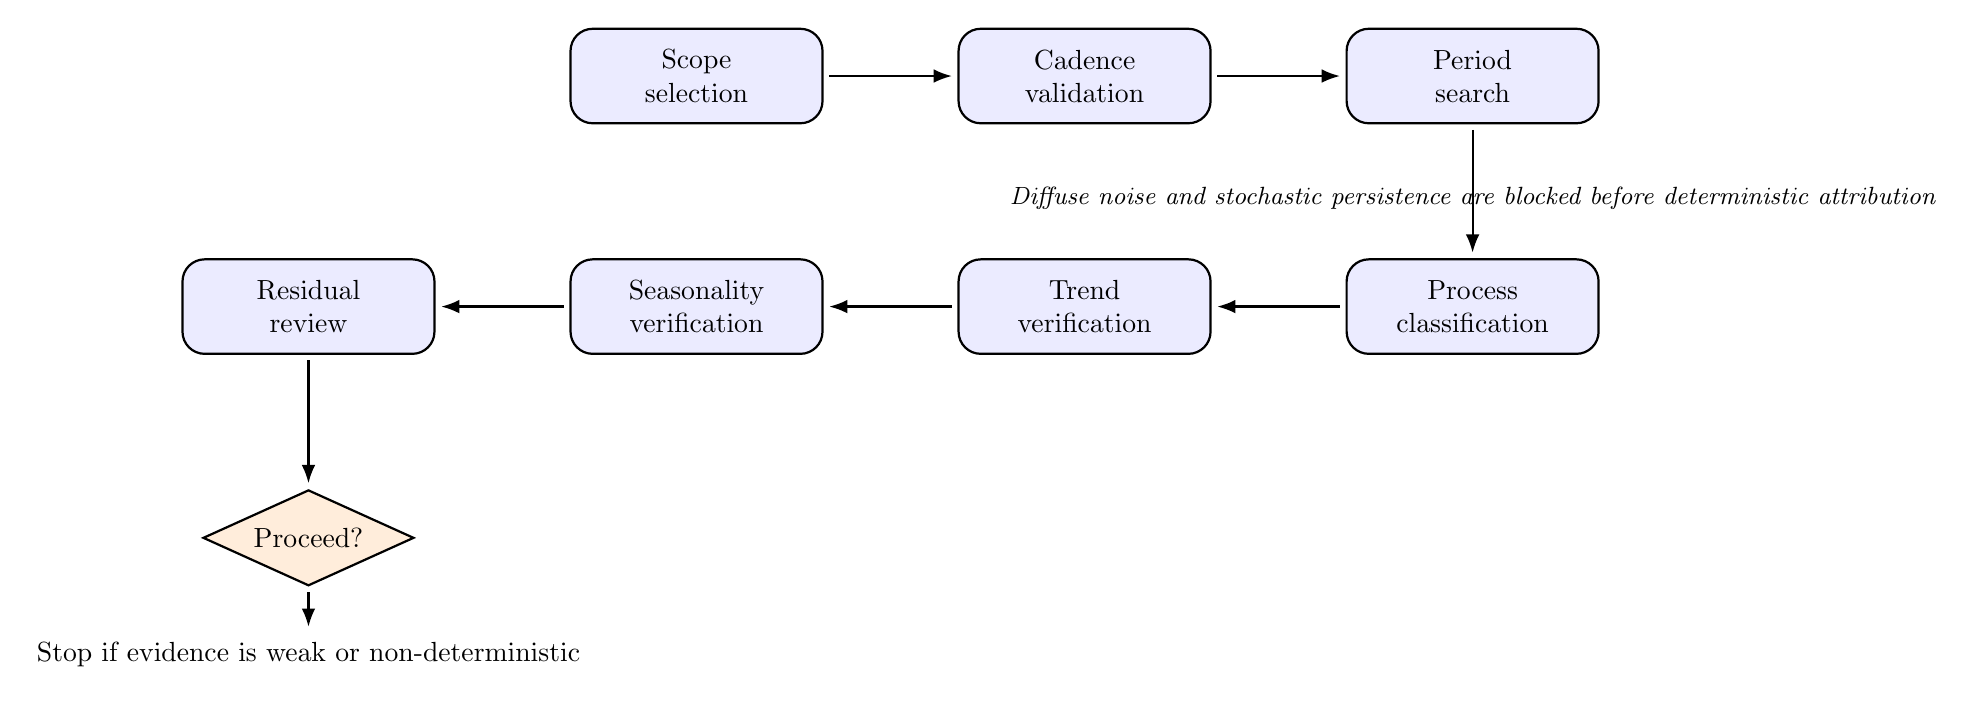
\begin{tikzpicture}[
  stage/.style={draw, rounded corners=8pt, align=center, minimum width=3.2cm, minimum height=1.2cm, fill=blue!8, line width=0.8pt},
  gate/.style={draw, diamond, align=center, aspect=2.2, fill=orange!14, line width=0.8pt},
  note/.style={font=\small\itshape, align=center},
  arrow/.style={-Latex, thick, shorten >=2pt, shorten <=2pt}
]

\node[stage] (scope) {Scope\\selection};
\node[stage, right=1.7cm of scope] (cadence) {Cadence\\validation};
\node[stage, right=1.7cm of cadence] (periods) {Period\\search};
\node[stage, below=1.7cm of periods] (classify) {Process\\classification};
\node[stage, left=1.7cm of classify] (trend) {Trend\\verification};
\node[stage, left=1.7cm of trend] (season) {Seasonality\\verification};
\node[stage, left=1.7cm of season] (resid) {Residual\\review};
\node[gate, below=1.7cm of resid] (decision) {Proceed?};

\draw[arrow] (scope) -- (cadence);
\draw[arrow] (cadence) -- (periods);
\draw[arrow] (periods) -- (classify);
\draw[arrow] (classify) -- (trend);
\draw[arrow] (trend) -- (season);
\draw[arrow] (season) -- (resid);
\draw[arrow] (resid) -- (decision);
\draw[arrow] (decision) -- ++(0,-1.2cm) node[below]{Stop if evidence is weak or non-deterministic};

\node[note, above=0.5cm of classify] {Diffuse noise and stochastic persistence are blocked before deterministic attribution};

\end{tikzpicture}
\end{document}
